\documentclass[a4paper,12pt]{article}
\usepackage{amsmath, amsthm, amssymb}
\usepackage{datetime}
\usepackage{framed}
\usepackage{enumitem}
\usepackage{fancyref}
\usepackage{wrapfig}
\usepackage{pifont}

\usepackage{csquotes}
\renewcommand{\mkbegdispquote}[2]{\itshape}

\usepackage{data/circledsteps}
\usepackage[top=1in,bottom=1in,left=1in,right=1in]{geometry} % 用于设置页面布局
\usepackage{xeCJK} % 用于使用本地字体
\usepackage[super, square, sort&compress]{natbib} % 处理参考文献
\usepackage{titlesec, titletoc} % 设置章节标题及页眉页脚
%\usepackage{xCJKnumb} % 中英文数字转换
\usepackage{amssymb}
\usepackage{amsmath} % 在公式中用\text{文本}输入中文
\usepackage{diagbox}
\usepackage{multirow} % 表格中使用多行
\usepackage{booktabs} % 表格中使用\toprule等命令
\usepackage{rotating} % 使用sidewaystable环境旋转表格
\usepackage{tabularx}
\usepackage{graphicx} % 处理图片
\usepackage{footnote} % 增强的脚注功能,可添加表格脚注
\usepackage{threeparttable} % 添加真正的表格脚注,示例见README
\usepackage{hyperref} % 添加pdf书签

\usepackage{tikz}
\usetikzlibrary{shapes,arrows,shadows}

% 字体设置
\setmainfont{Times New Roman}
\setsansfont[Scale=MatchLowercase,Mapping=tex-text]{PT Sans}
\setmonofont[Scale=MatchLowercase]{PT Mono}
\setCJKmainfont[ItalicFont={Kaiti SC}, BoldFont={Heiti SC}]{Songti SC}
\setCJKsansfont{Heiti SC}
\setCJKmonofont{Songti SC}
% \setCJKmainfont[BoldFont={FZXiaoBiaoSong-B05S}]{Songti SC}
% \setCJKfamilyfont{kai}[BoldFont=Heiti SC]{Kaiti SC}
% \setCJKfamilyfont{song}[BoldFont=Heiti SC]{Songti SC}
% \setCJKfamilyfont{hei}[BoldFont=Heiti SC]{Heiti SC}
% \setCJKfamilyfont{fsong}[BoldFont=Heiti SC]{Songti SC}
% \newcommand{\kai}[1]{{\CJKfamily{kai}#1}}
% \newcommand{\hei}[1]{{\CJKfamily{hei}#1}}
% \setromanfont[Mapping=tex-text]{TeXGyrePagella}
% \setsansfont[Scale=MatchLowercase,Mapping=tex-text]{TeXGyrePagella}
% \setmonofont[Scale=MatchLowercase]{Courier New}
%%设置常用中文字号,方便调用
\newcommand{\erhao}{\fontsize{22pt}{\baselineskip}\selectfont}
\newcommand{\xiaoerhao}{\fontsize{18pt}{\baselineskip}\selectfont}
\newcommand{\sanhao}{\fontsize{16pt}{\baselineskip}\selectfont}
\newcommand{\xiaosanhao}{\fontsize{15pt}{\baselineskip}\selectfont}
\newcommand{\sihao}{\fontsize{14pt}{\baselineskip}\selectfont}
\newcommand{\xiaosihao}{\fontsize{12pt}{\baselineskip}\selectfont}
\newcommand{\wuhao}{\fontsize{10.5pt}{\baselineskip}\selectfont}
\newcommand{\xiaowuhao}{\fontsize{9pt}{\baselineskip}\selectfont}
\newcommand{\liuhao}{\fontsize{7.5pt}{\baselineskip}\selectfont}

% 章节标题显示方式及页眉页脚设置
% \item xCJKnumb是自己额外安装的包
% \item titleformat命令定义标题的形式
% \item titlespacing定义标题距左、上、下的距离
\titleformat{\section}{\raggedright\large\bfseries}{\thesection}{1em}{}
\titleformat{\subsection}{\raggedright\normalsize\bfseries}{\thesubsection}{1em}{}
\titlespacing{\section}{0pt}{*0}{*2}
\titlespacing{\subsection}{0pt}{*0}{*1}
% 由于默认的2em缩进不够,所以我手动调整了,但是在windows下似乎2.2就差不多了,或者是article中没有这个问题
\setlength{\parindent}{2.2em}

% 设置表格标题前后间距
\setlength{\abovecaptionskip}{0pt}
\setlength{\belowcaptionskip}{0pt}


\renewcommand{\refname}{\bfseries{参~考~文~献}} %将Reference改为参考文献(用于 article)
% \renewcommand{\bibname}{参~考~文~献} %将bibiography改为参考文献(用于 book)
\renewcommand{\baselinestretch}{1.38} %设置行间距
\renewcommand{\figurename}{\small\ttfamily 图}
\renewcommand{\tablename}{\small\ttfamily 表}


\usepackage{stmaryrd}
\usepackage{mathtools}


\title{论“自然语言编程”的不智}
\date{1978 年}
\author{Edsger W. Dijkstra}

\begin{document}

\maketitle{}

从自动计算的早期开始,总有人认为编程必须如同使用任何形式符号体系那样的精确与谨慎是一种缺陷。他们批评机器对于其执行的指令过于严格的服从性,哪怕稍加思考就能发现这些指令明显错误。正如A.E.Houseman所说:“但一刻钟对于思考来说是很长的时间,而思考本身是个痛苦的过程。” 他们热切地期待并寻找那些更智能的机器,它们能拒绝执行明显愚蠢的任务,如小错误引发的活动。

\begin{figure}[ht]
    \centering
    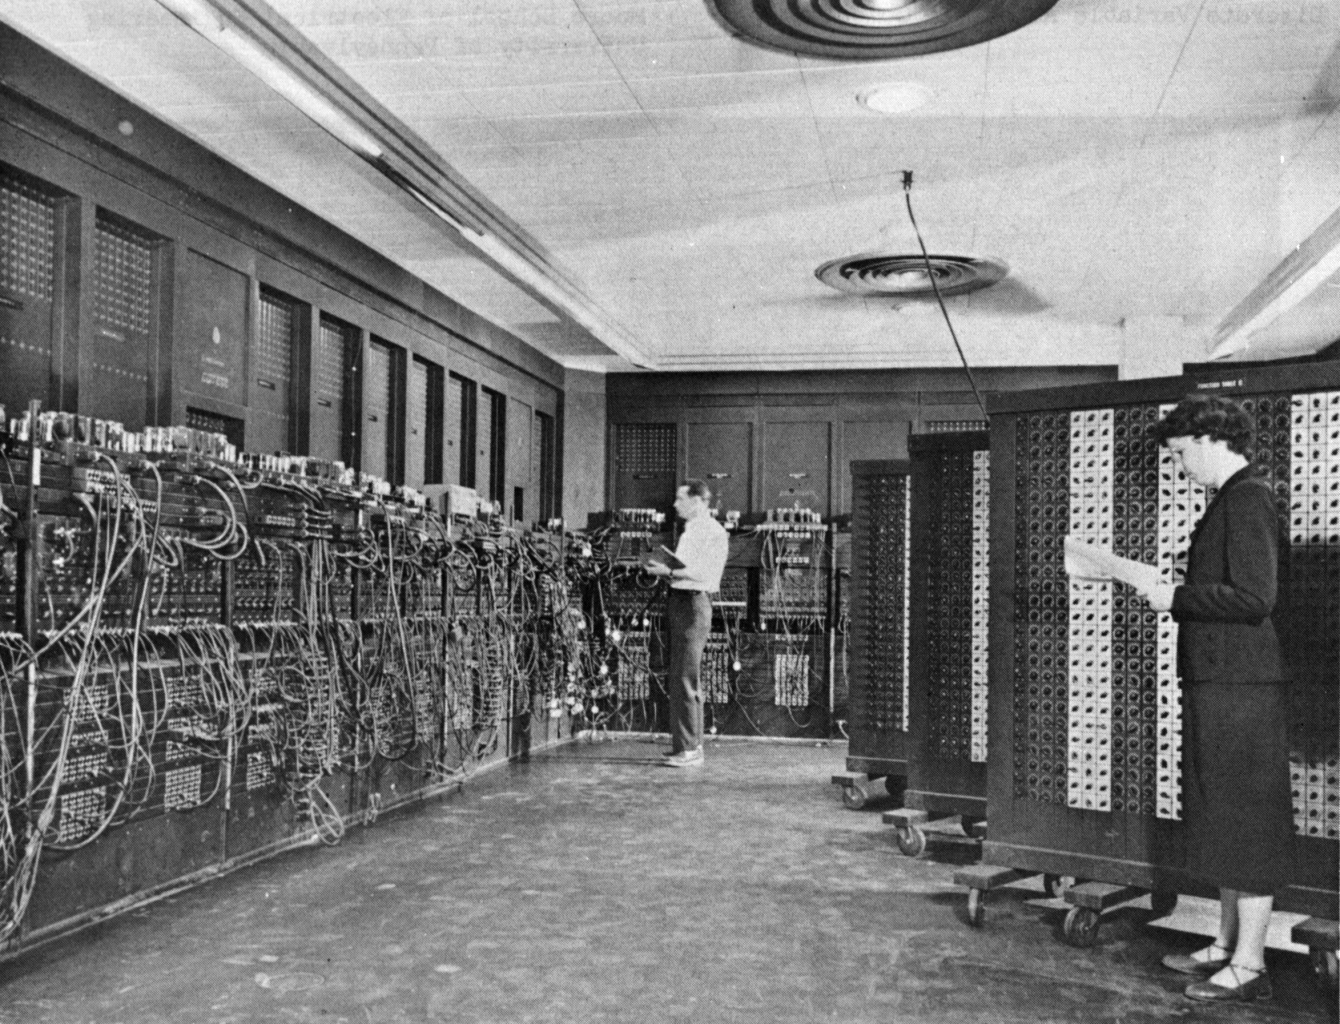
\includegraphics[height=2.5in]{images/ENIAC.jpeg}
    \caption{世界上第一台计算机 ENIAC}
\end{figure}

机器代码,由于几乎不包含任何冗余,很快就被认为是人与机器之间不必要的风险界面。部分作为对这种看法的回应,所谓的“高级编程语言”应运而生,随着时间的推移,我们学会了在一定程度上增强了对愚蠢错误的防护。一个重要的进步是,现在许多愚蠢的错误将导致错误信息的产生,而不是错误的结果。(甚至这种改进并不是普遍受欢迎:有些人发现无法忽略的错误信息比错误的结果更令人烦恼,而在评价编程语言的相对优势时,一些人仍然倾向于将“编程的简易度”与犯下未被察觉错误的容易度相等同。)然而,与编程语言相对应的(抽象)机器仍然是一个忠实的奴隶,即那种完全能够执行无意义指令的非理性自动机。编程仍然是使用形式化的符号体系,因此,依旧需要之前所要求的那种精确和谨慎。

\begin{wrapfigure}{r}{0.35\textwidth}
    \centering
    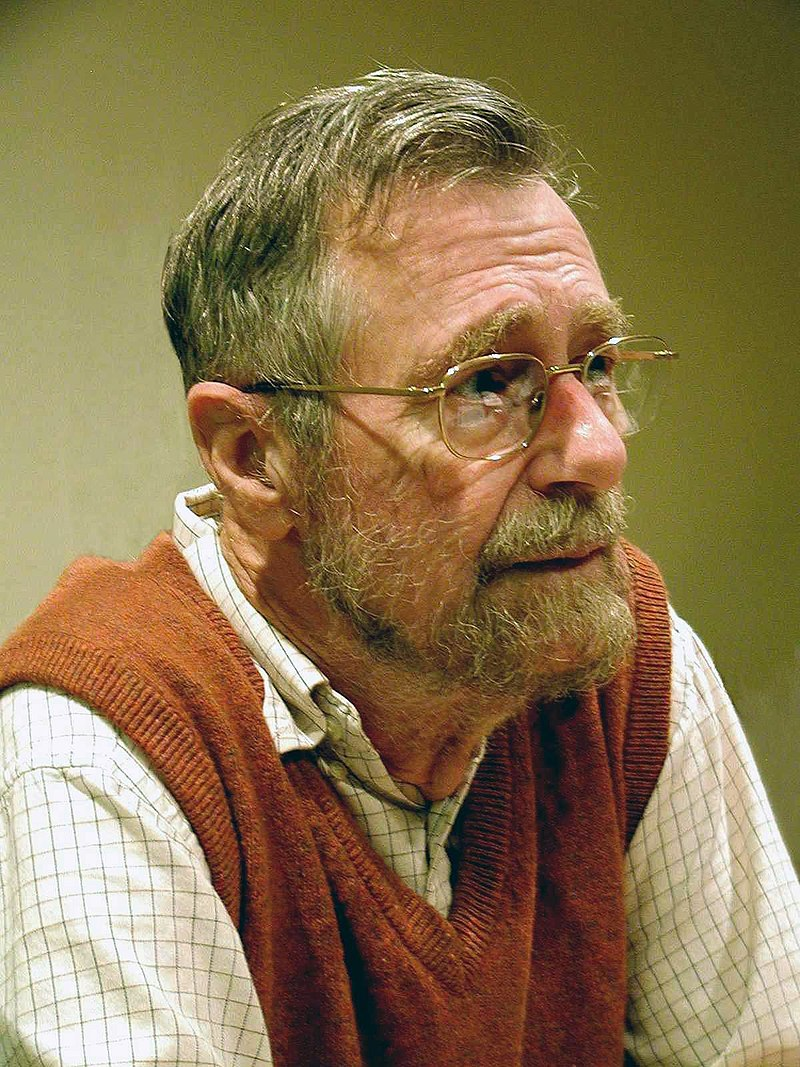
\includegraphics[height=2.2in]{images/Edsger_Wybe_Dijkstra.jpeg}
    \caption{Edsger W. Dijkstra}
\end{wrapfigure}

为了让机器使用更加简便,有人提出了一个想法:(尝试)设计可以接受我们用母语发出的指令的机器。诚然,这会让机器变得更复杂,但有人辩称,通过让机器承担更重的负担,我们的生活将变得更轻松。如果你认为使用形式符号体系是造成困难的根源,这看起来似乎合理。但这个论点真的成立吗?我对此表示怀疑。

我们现在明白,选择一个界面不仅仅是(固定数量的)工作分配问题,因为还必须考虑界面上进行协作和交流所涉及的工作。根据我们的实际经验—我不得不说,这是一种警醒的体验—我们知道,改变界面很容易在界面两侧都增加工作量(有时甚至是极大的增加)。因此,现在更倾向于使用所谓的“狭窄界面”。所以,变成用人类的母语进行机器与人的交流会大幅增加机器的负担,我们还是不得不对这样做会简化人类生活的假设提出质疑。

\begin{figure}[ht]
    \centering
    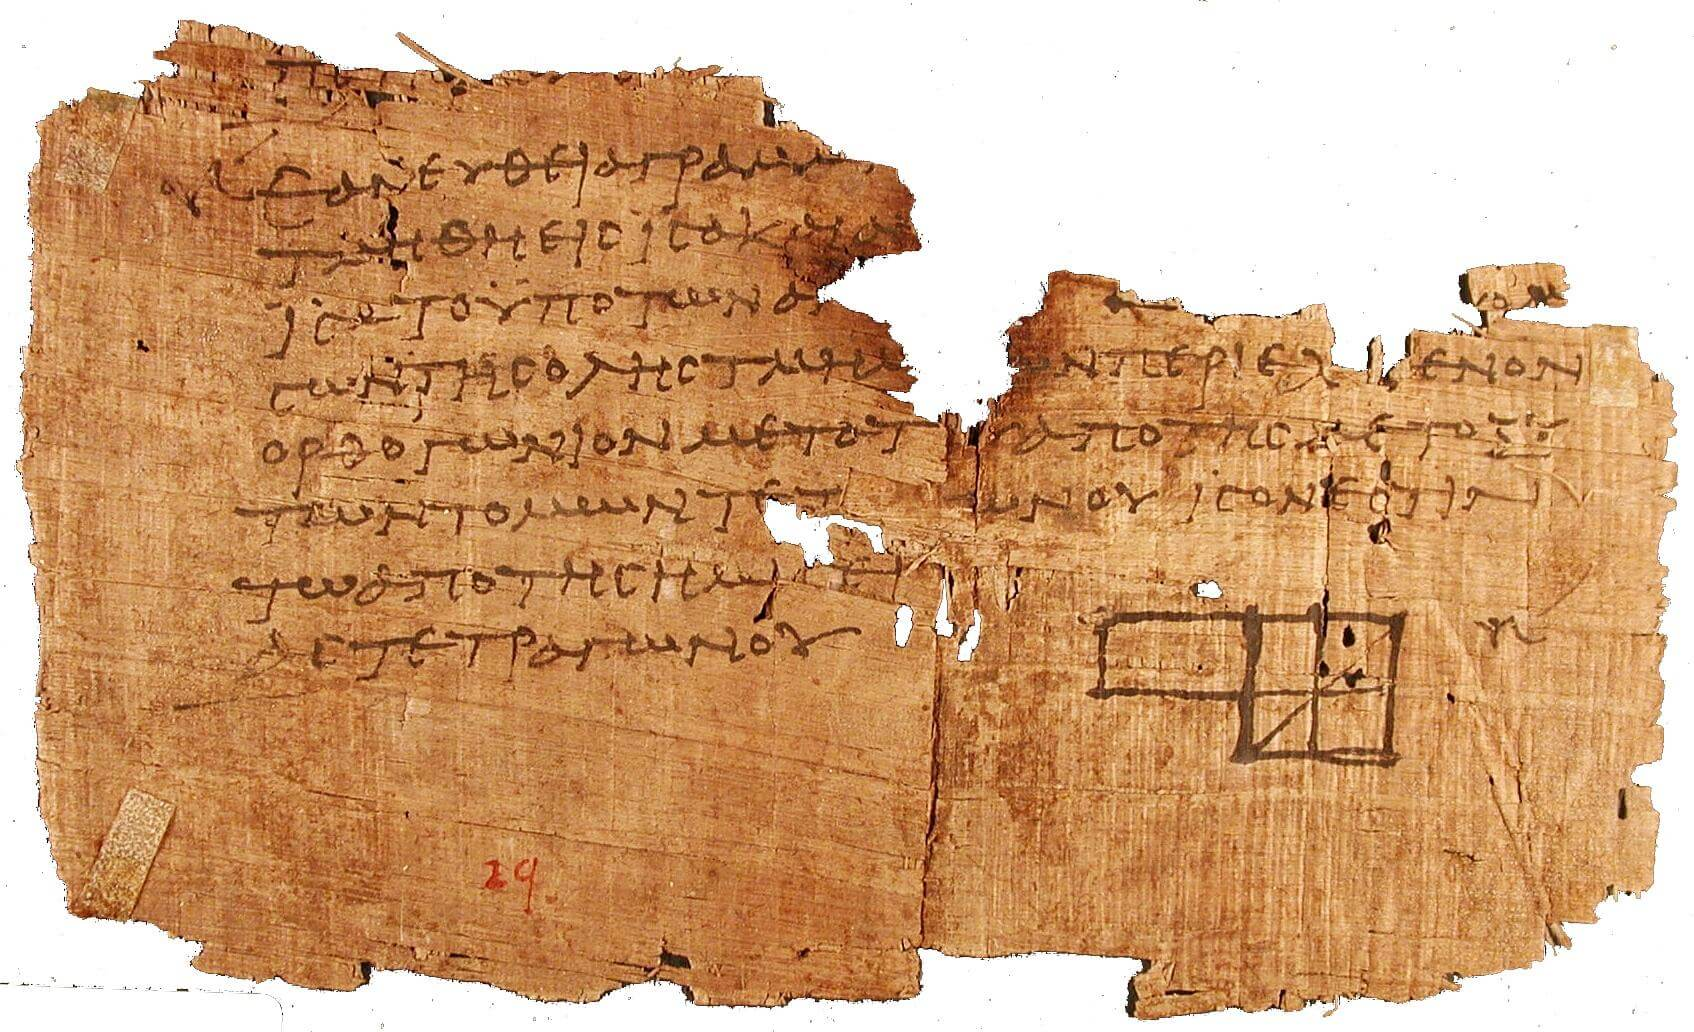
\includegraphics[height=2.5in]{images/elements.jpeg}
    \caption{《几何原本》残片}
\end{figure}

简单回顾数学史就能证明这种挑战有多么有道理。希腊数学之所以停滞不前,是因为它一直停留在口头和图像化的层面上;穆斯林的“代数”在尝试使用符号之后变得胆怯,当它回归修辞风格时便走向了衰亡。现代文明世界能够出现—无论是好是坏—是因为西欧能够摆脱中世纪经院哲学的枷锁—那是对语言精确性的徒劳尝试!—这要归功于像 Vieta、Descartes、Leibniz 和(后来的)Boole等人精心设计或至少是有意识设计的形式符号。

\begin{figure}[ht]
    \centering
    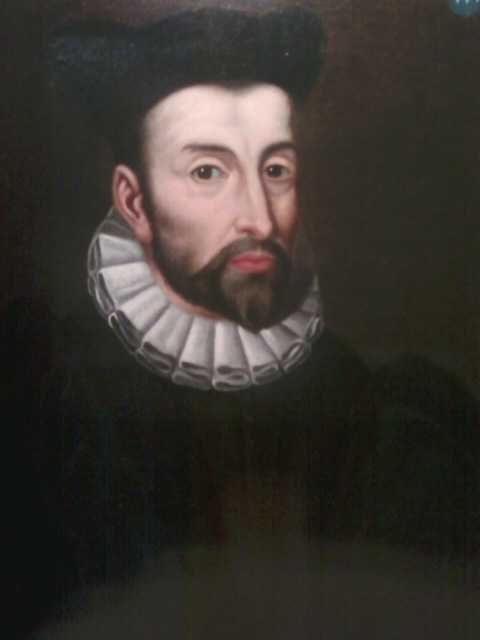
\includegraphics[height=1.5in]{images/Francois_Viete.jpeg}
    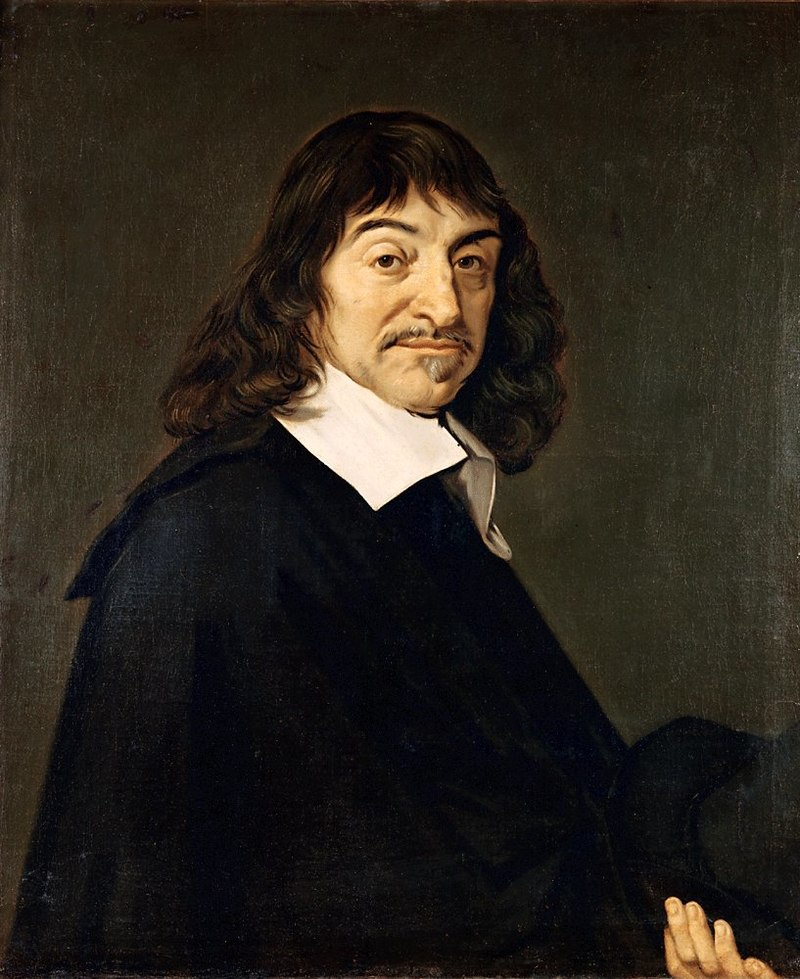
\includegraphics[height=1.5in]{images/Descartes.jpeg}
    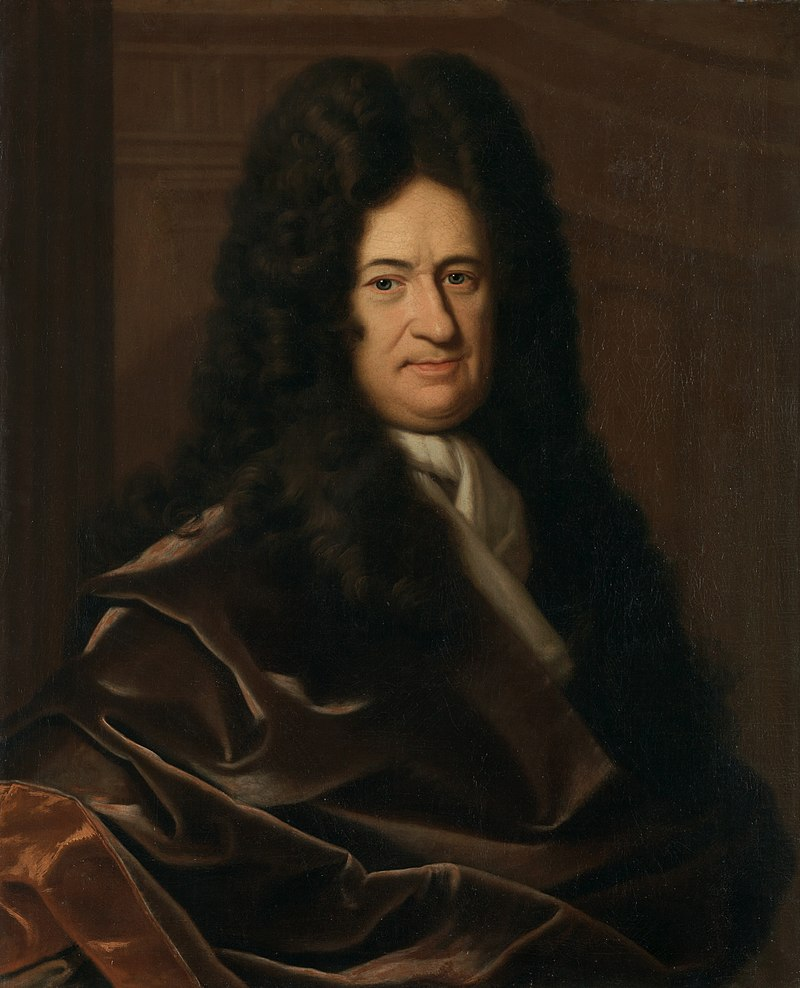
\includegraphics[height=1.5in]{images/Leibniz.jpeg}
    \caption{Vieta、Descartes、Leibniz 像}
\end{figure}

形式文本的优点在于,它们的操作要合法,只需遵守一些简单的规则。仔细想想,你会发现它们是一种极其有效的工具,能够排除各种荒谬,这些荒谬在我们使用母语时几乎是不可避免的。

我们不应将使用形式符号看作一种负担,反而应将使用它们的便利视为一种特权:得益于它们,学生们能够学会做过去只有天才才能完成的事情。(显然,这点并没有被1977年在一份技术报告前言中写到的作者理解,他甚至为了所谓的“清晰”,避免使用逻辑连接符的标准符号。这句话的出现表明,这种误解并不仅限于他一人。)总而言之,我们使用母语的“自然”实质上就是我们轻易地使用它们来发表那些荒谬的言论的能力。
\footnote{由于教育趋势偏离了智力训练,过去几十年来,在西方世界,人们对自己语言的掌握程度显著下降:许多按上一代标准来看应该更懂得的人,现在已经无法有效使用自己的母语,即使是在它相当适用的情况下也是如此。(你只需要看看科学文章、技术报告、政府出版物等中那些令人担忧的、在仔细阅读后显得毫无意义的冗长文字。)这一现象—被称为“新文盲”—应当让那些缺乏足够技术洞察力来预测其失败的自然语言编程的信徒们感到泄气。}

\begin{figure}[ht]
    \centering
    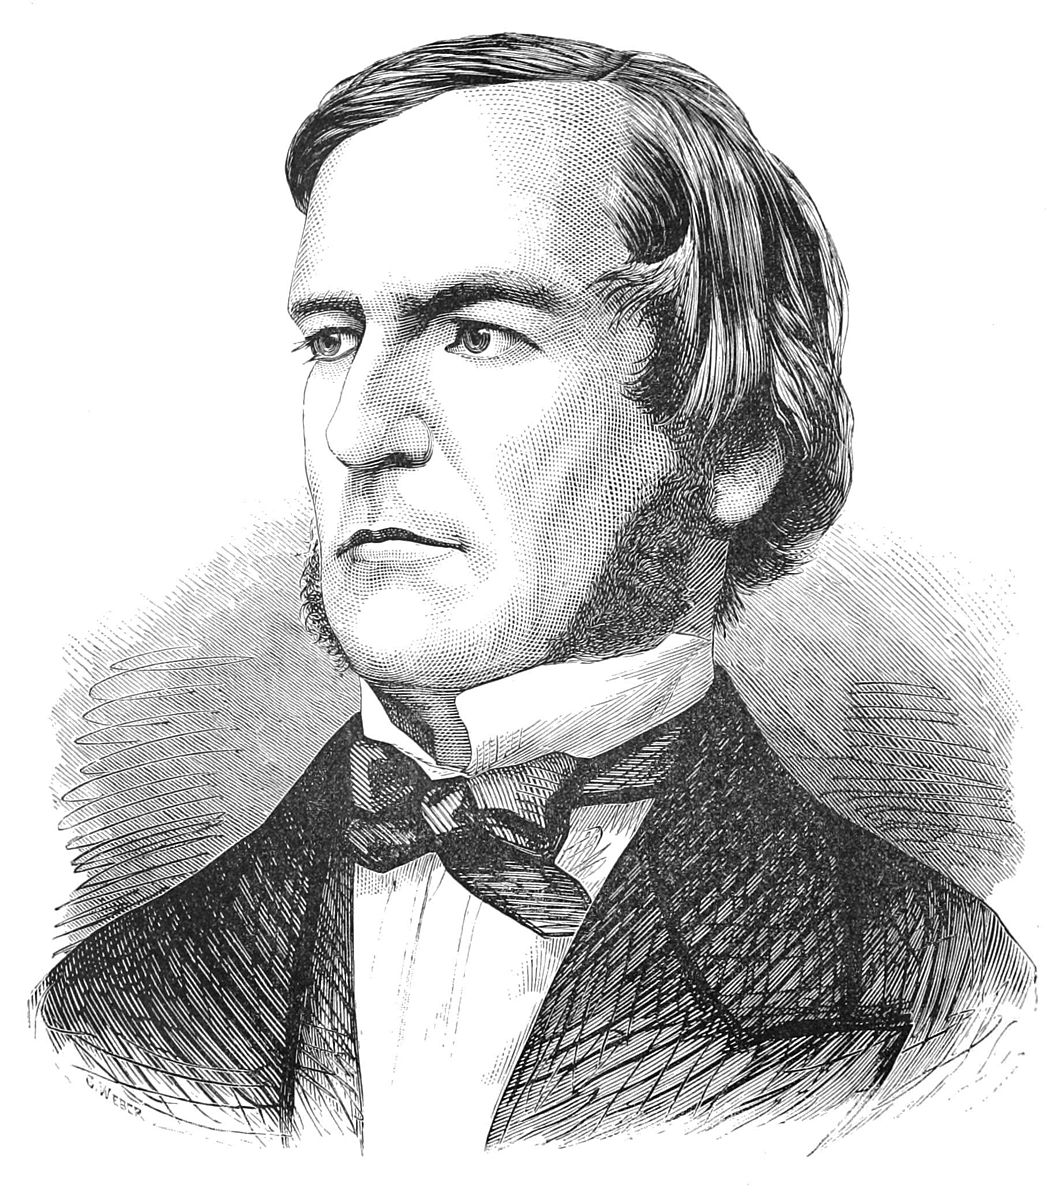
\includegraphics[height=2.5in]{images/George_Boole.jpeg}
    \caption{George Boole 像}
\end{figure}

尝试想象一下,如果从一开始我们的母语就成为我们信息处理设备的唯一输入和输出方式,可能会有一些启发。我经过深思熟虑的猜想是,历史在某种意义上可能会重演,计算机科学主要将是一种确实深奥的艺术,即如何从那里引导出一个定义足够明确的形式系统。我们将需要动用全世界的智力来使界面足够窄,从而使其可用,并且考虑到人类的历史,猜测要做到足够好可能还需要几千年的时间,这并不是过于悲观的想法。

我从如下这种强烈的直觉中获得了许多安慰:我怀疑,无论是用荷兰语、英语、美式英语、法语、德语还是斯瓦希里语来编程的机器,它们的制造难度和使用难度都同样巨大。

 \\Plataanstraat 5\\
5671 AL NUENEN\\
荷兰 Edsger W.Dijkstra 教授博士\\
Burroughs 研究员\\




\end{document}


